\section{研究内容与技术路线}
\label{section-tech}

针对现有控制系统在设计与验证阶段面临的挑战，并为实现\ref{section-bg-target}节所述的研究目标，本论文的核心工作聚焦于构建一个由大语言模型（LLM）驱动的、覆盖控制系统状态机模型"生成-验证-修复"全生命周期的自动化、迭代式闭环方法。该方法旨在系统性地解决从非形式化需求到高可信度模型的转化难题，通过深度融合大语言模型强大的自然语言理解、代码生成与逻辑推理能力，为复杂控制系统的功能安全提供坚实的技术支撑。本论文的研究工作可系统地划分为四个紧密衔接的研究方向，其相互关系如图\ref{fig:methodology}所示。

\begin{figure}[h]
    \centering
    \includegraphics[width=0.95\textwidth]{figs/任务架构.drawio.pdf}
    \caption{基于大语言模型（LLM）的控制系统模型迭代式精化方法示意图}
    \label{fig:methodology}
\end{figure}

首先，为应对复杂控制系统需求向形式化模型精确转化的挑战，第\ref{section-tech-generation}节的研究内容一将提出一种基于控制系统软件需求的LLM状态机结构化建模方法。该方法将大语言模型作为核心引擎，旨在实现对非形式化的系统需求文档进行深度语义解析，自动生成一个初始的状态机模型。该研究的最终目标是直接构建一个结构完整且语义精确的状态机模型，从而为整个闭环方法奠定坚实的基础，即一个高质量的初始模型。

其次，为了确保后续验证过程的有效性与针对性，第\ref{section-tech-vergeneration}节的研究内容二致力于解决验证资产（Verification Assets）的自动化生成问题，提出一种基于模型元素的验证场景与待验证性质生成方法。此方法将综合分析研究内容一所生成模型中的关键元素（如状态、转移、事件等），并结合原始需求文档，特别是其中蕴含的时间性质（Temporal Properties）等关键非功能性需求，利用大语言模型生成一组高覆盖度的验证剖面（Verification Profiles）与相应的、可形式化的待验证性质规约。

再次，传统的模型验证方法往往依赖于严格的形式化规约，实施成本高昂且难以覆盖所有关键行为。为解决此问题，第\ref{section-tech-verification}节的研究内容三将探索一种基于验证剖面的状态机验证方法。该方法以研究内容二生成的验证剖面为驱动，通过模拟执行（Simulation）或模型检测（Model Checking）等技术，对当前状态机模型的行为进行检验。此方法聚焦于关键业务场景，旨在高效地检测出模型在特定场景下与预期性质不符的缺陷（Defects），尤其关注那些与实时性、并发性相关的动态行为偏差。

最后，为了实现模型的自我完善与收敛，形成一个完整的反馈闭环，第\ref{section-tech-fix}节的研究内容四将聚焦于基于已知验证缺陷的模型迭代修复方法。该方法以研究内容三检测到的缺陷作为输入，结合当前模型状态与待满足的性质，运用大语言模型的代码生成与逻辑修正能力，对状态机模型进行自动化修复，形成一个更优的新版本模型。通过将上述四个研究内容有机地组织成一个迭代循环，该方法能够反复进行"验证-缺陷检测-修复"的过程，直至模型在所有验证剖面下均表现出稳定且正确的行为，最终获得一个高可信、满足复杂控制需求的系统模型。

\subsection{研究内容一：基于控制系统软件需求的LLM状态机结构化建模方法}
\label{section-tech-generation}

本研究旨在解决控制系统状态机建模过程中从非结构化需求描述到精确模型转化的复杂性与挑战。针对这一核心问题，我们提出一种基于大语言模型（LLM）辅助的多步式建模方法，该方法实现从高层级需求到完整、精确状态机模型的自动化构建，并确保模型与控制系统特有的时间属性和动态行为的精确对应。

本方法利用LLM强大的自然语言理解与生成能力，对控制系统自然语言需求文档进行深度解析，自动生成初步的状态机模型。这一过程旨在弥合自然语言描述与形式化模型之间的语义鸿沟，为后续的验证与修复奠定基础。考虑到控制系统对时间属性和实时性的严格要求，模型生成阶段将特别关注需求中蕴含的时间约束，例如事件的触发时序、状态的持续时间以及响应的截止时间等。LLM通过对这些时间性质的识别与建模，确保生成的状态机模型能够准确反映系统的动态行为。相关研究表明，LLM在自动化控制系统设计方面展现出巨大潜力 \upcite{guo2024controlagent}，尤其是在处理复杂需求和生成初始模型方面 \upcite{tsai2024using}。

具体而言，模型生成过程可形式化表示为函数 $G$，其输入为控制系统需求 $R$，输出为状态机模型 $M$：
\begin{equation}
M = G(R)
\label{eq:model_generation}
\end{equation}
其中，$R$ 是一组自然语言描述的控制系统功能与非功能性需求，可能包含对时间、并发、同步等方面的约束。$M$ 是一个形式化的状态机模型，其结构包括状态集合 $S$、事件集合 $E$、变量集合 $V$、迁移集合 $Tr$ 和动作集合 $A$。即 $M = (S, E, V, Tr, A)$。模型 $M$ 的生成过程可进一步分解为一系列子任务，每个子任务都由LLM驱动完成，以确保模型构建的准确性和完整性。

在模型生成过程中，LLM将执行以下关键步骤。首先是需求解析与元素识别：LLM对输入需求 $R$ 进行语义解析，识别出控制系统中的核心实体，包括但不限于系统可能存在的各种状态（如"运行中"、"停止"、"故障"等）、触发状态转换的事件（如"启动信号"、"传感器数据到达"、"定时器超时"等）以及系统内部用于记录和控制行为的变量（如"温度值"、"速度设定"、"计数器"等）。这一阶段尤其注重从需求描述中提取与时间相关的实体，例如"每隔500ms"、"在10秒内完成"等，以捕捉实时系统的关键特性 \upcite{pku2019realtime, buaa2015timeautomata}。

其次是状态机结构构建：在识别出基本元素后，LLM根据需求中描述的逻辑关系，构建状态之间的迁移。每个迁移 $tr \in Tr$ 可形式化定义为四元组 $(s_\text{src}, e, g, s_\text{dst})$，其中 $s_\text{src} \in S$ 是起始状态，$s_\text{dst} \in S$ 是目标状态，$e \in E$ 是触发事件，$g \in Guard(V)$ 是基于变量的守卫条件函数。守卫条件 $g$ 通常是基于系统变量的布尔表达式，例如"温度 > 100"或"计数器 < 5"，其形式化表示为 $g: V \rightarrow \{\text{true}, \text{false}\}$。对于控制系统，守卫条件中常常包含时间相关的判断，如"距离上次事件发生超过5秒"，可形式化为 $g_{\text{time}}(v) = (v_{\text{last\_event}} + \Delta t < v_{\text{current\_time}})$。状态集合 $S$ 的构建遵循层次化原则，允许复合状态 $s_c = \{s_\text{sub1}, s_\text{sub2}, \dots\}$ 包含子状态，以表达复杂系统的运行模式。

再次是动作与时间属性关联：LLM将识别出的动作 $a \in A$ 与相应的状态进入/退出、迁移触发等时机进行关联。每个动作 $a$ 可表示为 $a: V \rightarrow V$ 的状态转换函数。动作可以是变量的赋值、外部设备的控制指令或内部事件的生成。特别地，LLM会根据需求中的时间约束，为状态或迁移添加时间属性。例如，为状态 $s \in S$ 定义最小持续时间 $t_{\min}(s)$ 和最大持续时间 $t_{\max}(s)$，形式化为状态不变式 $Inv(s) = [t_{\min}, t_{\max}]$；为迁移 $tr \in Tr$ 定义最晚触发时间 $t_{\text{deadline}}(tr)$。这些时间属性的引入，使得生成的状态机模型能够捕捉控制系统的实时行为特征 \upcite{csdn2021control}。

最后是模型输出与形式化表示：LLM将上述识别和构建的元素整合，生成符合特定形式化语言（如SCXML或其他自定义状态机描述语言）的状态机模型文本。此阶段确保输出模型的语法正确性与语义完整性，为后续的验证与分析提供可操作的输入。

图\ref{fig:model_generation_diagram}示意了基于LLM辅助的模型生成过程，展示了从自然语言需求到形式化状态机模型的转化流程。

\begin{figure}[h!]
    \centering
    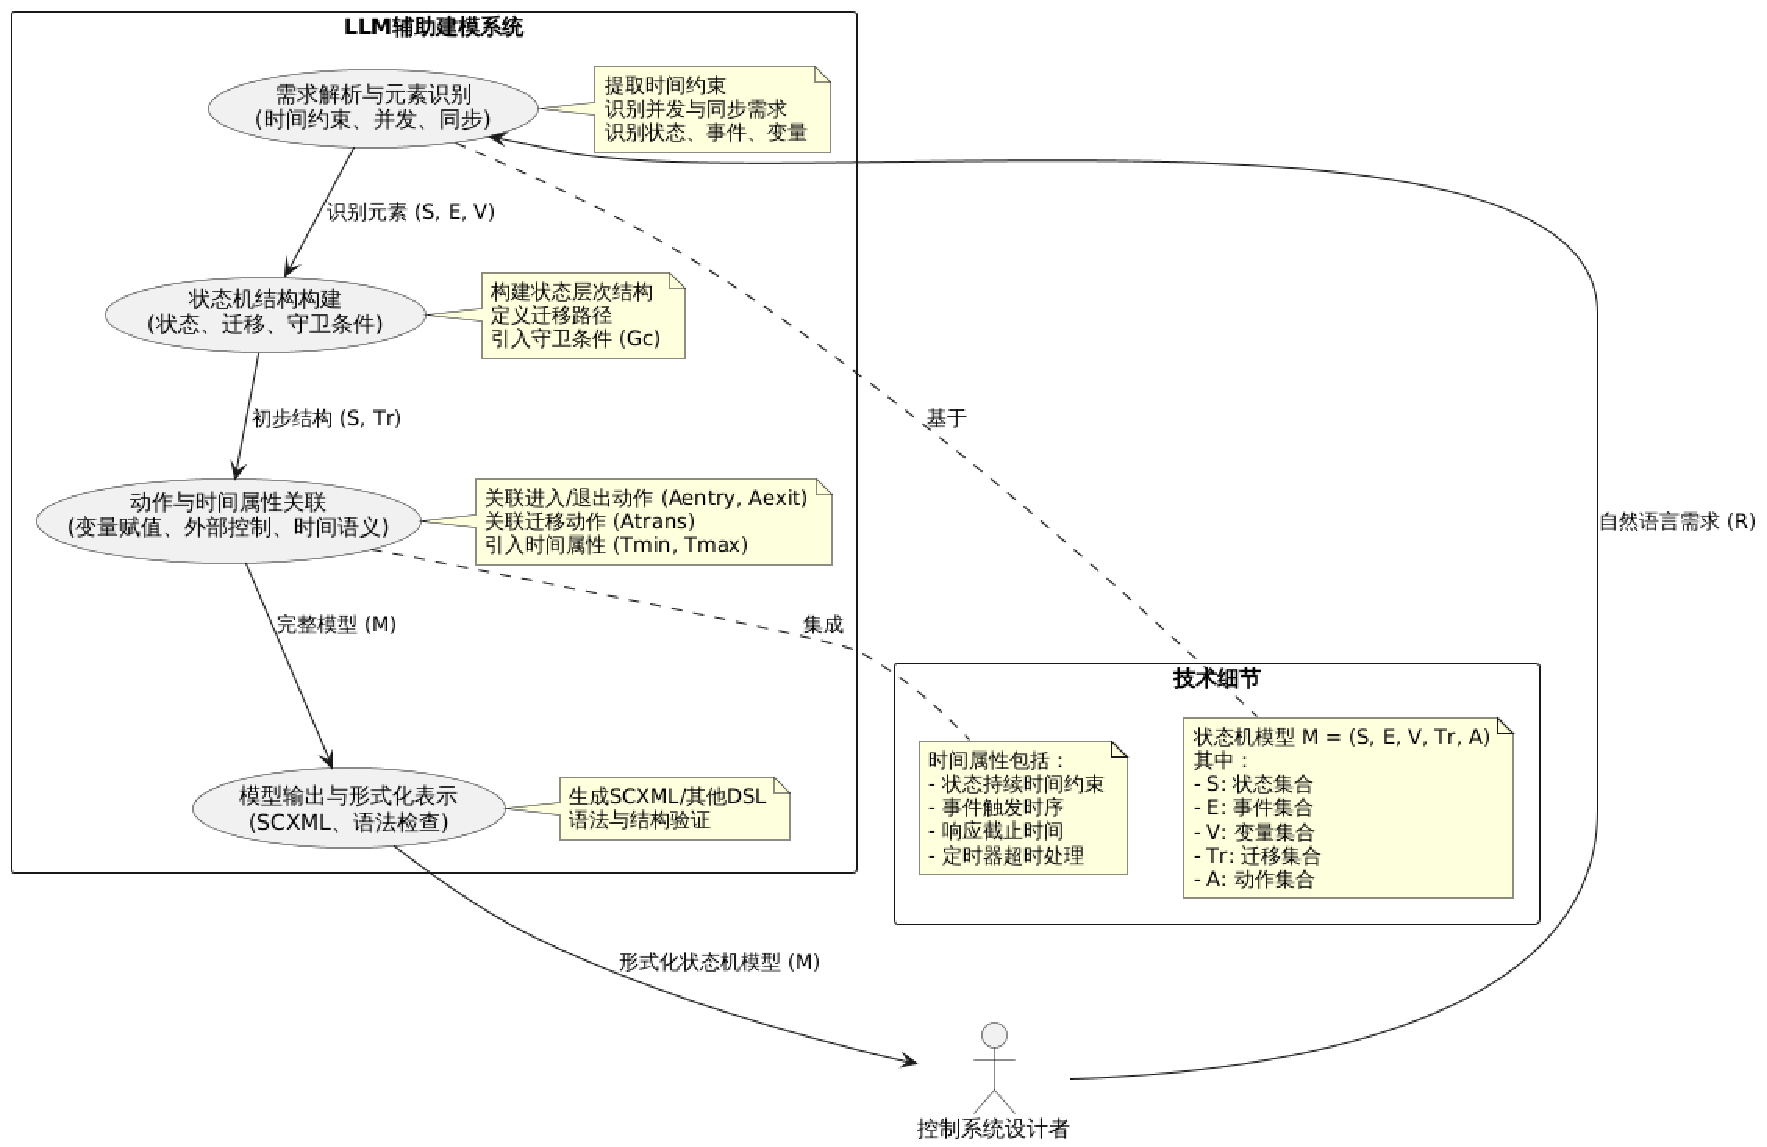
\includegraphics[width=1.0\textwidth]{figs/model_generation_enhanced.png}
    \caption{基于LLM辅助的控制系统模型生成示意图}
    \label{fig:model_generation_diagram}
\end{figure}

\subsection{研究内容二：基于模型元素的验证场景与待验证性质生成方法}
\label{section-tech-vergeneration}

在复杂控制系统设计与验证过程中，传统方法在生成全面且高质量的验证场景与待验证性质方面面临诸多挑战。尤其是在面对控制系统特有的时间属性和并发行为时，手动生成能够充分覆盖关键路径、边界条件及异常情况的验证资产，不仅耗时耗力，且极易遗漏潜在缺陷。针对这一痛点，本研究提出一种基于模型元素的验证场景与待验证性质生成方法，旨在通过深度融合大语言模型（LLM）的语义理解与推理能力、控制系统领域知识以及状态机模型结构信息，实现验证资产的自动化、智能化生成，从而显著提升验证效率与覆盖度。

本方法的核心思想在于，将控制系统需求文档、已构建的状态机模型以及外部领域知识作为综合输入，利用LLM作为处理引擎的自然语言处理能力，从非形式化的需求描述中精准提取关键信息，并结合模型元素的结构化特征，自动构建用于模型验证的验证剖面（Verification Profile）和形式化性质（Formal Properties）。这里，外部领域知识特指从控制系统领域文档、标准、协议或设计规范中提取的结构化知识，以确保生成内容的准确性和可靠性，避免依赖LLM内部可能存在的泛化或不确定知识。本方法尤其关注控制系统对时间属性的严格要求，确保生成的验证内容能够全面反映系统的实时性、并发性及顺序性约束。通过这种方式，我们旨在克服传统测试方法在覆盖度上的局限性，并降低形式化验证对人工专业知识的依赖，为后续高效、高可信度的模型验证奠定基础。

具体而言，本方法将验证剖面定义为一系列有序的事件序列与系统状态约束的集合，它描述了系统在特定操作情境下的预期行为轨迹。形式上，一个验证剖面 \( SP \) 可以表示为：
$$ SP = \langle (E_1, C_1, \tau_1), (E_2, C_2, \tau_2), \dots, (E_n, C_n, \tau_n) \rangle $$
其中，\( E_i \) 代表在时间点 \( t_i \) 发生的事件或输入，\( C_i \) 代表在事件 \( E_i \) 发生时系统所应满足的状态约束或条件，\( \tau_i \) 代表与事件 $E_i$ 或状态 $C_i$ 相关的时间约束区间。这些事件可以包括外部触发、内部信号、时间流逝等，而状态约束则涉及控制变量的取值范围、系统所处模式等。LLM将根据需求文档中对系统行为的描述，识别出关键的事件触发条件、状态迁移路径以及时间限制，并将其转化为结构化的验证剖面。例如，对于一个飞行控制系统，一个验证剖面可能描述为："当飞机处于起飞模式且速度达到 $V_{\text{takeoff}}$ 时，起落架收回事件 $E_{\text{gear\_retract}}$ 发生，且系统应在 $ [t_{\text{min}}, t_{\text{max}}] $ 时间内进入爬升状态 $S_{\text{climb}}$。"

同时，本方法将待验证性质定义为对状态机模型行为的逻辑断言，用于检验模型是否满足特定的功能安全要求。这些性质主要分为安全性质（Safety Properties）和活性性质（Liveness Properties），并特别强调时间性质（Temporal Properties）。安全性质确保"坏事永远不会发生"，例如"系统永远不会同时处于起飞模式和降落模式"。活性性质确保"好事最终会发生"，例如"在接收到启动指令后，系统最终会进入运行状态"。时间性质则涉及事件发生的时序关系和时间约束，例如"从刹车指令发出到刹车动作完成，时间间隔不超过 $T_{\text{max}}$"。本研究将利用LLM从需求中识别这些隐式或显式的性质，并将其形式化为时序逻辑表达式，例如线性时序逻辑（LTL）或计算树逻辑（CTL）的变体，并特别引入时钟变量和时间区间来精确表达控制系统的时间特性。形式上，一个时间性质 $P$ 可以表示为：
$$ P = \text{AG}(S_{\text{mode1}} \implies \text{AF}_{\le T_{\text{limit}}}(S_{\text{mode2}})) $$
其中，$ \text{AG} $ 表示"全局总是"，$ \text{AF}_{\le T_{\text{limit}}} $ 表示"最终会在 $T_{\text{limit}}$ 时间内发生"，$ S_{\text{mode1}} $ 和 $ S_{\text{mode2}} $ 代表特定的系统状态。LLM将通过分析需求文档中的时序描述、性能指标以及安全规范，生成此类形式化性质。例如，对于一个电机控制系统，可能生成性质："在电机启动后，转速必须在 $t_{\text{startup}}$ 时间内达到额定转速，且在运行过程中，转速波动不能超过 $ \pm \delta $。"

待验证性质的元模型可以定义为一个四元组，如下所示：
\begin{equation}
Property = (Type, Scope, Predicate, TemporalConstraint)
\label{eq:property_model}
\end{equation}
其中，$Type$是性质的类型，可以是安全性质（Safety）、活性性质（Liveness）或时间性质（Temporal）；$Scope$是性质的作用范围，指明该性质适用于模型的哪个部分或在何种条件下进行验证，例如全局（Globally）、在某个状态下（OnState）、在某个事件发生后（AfterEvent）等。$Predicate$是性质的核心逻辑断言，通常是一个布尔表达式，描述了系统变量、状态或事件之间的关系，例如，$ (Temperature \ge T_{\text{min}} \land Temperature \le T_{\text{max}}) $ 或 $ (MotorState = Running) $；$TemporalConstraint$是时间约束，用于精确表达事件发生或状态持续的时间关系。这可以是一个时间区间 $ [t_{\text{min}}, t_{\text{max}}] $，表示某个事件必须在 $t_{\text{min}}$ 到 $t_{\text{max}}$ 时间内发生，或者某个状态必须持续在该时间区间内。例如，$ \text{AF}_{\le T_{\text{limit}}} $ 中的 $ T_{\text{limit}} $ 即为时间约束。

为了实现上述验证剖面和形式化性质的自动化生成，本方法将构建一个多阶段的生成流程，如图 \ref{fig:verification_generation_flow} 所示。在此流程中，大语言模型（LLM）被明确定义为一个可控的、定向的处理引擎，其核心能力被引导至执行一系列特定的子任务，而非作为一个模糊的知识黑箱。首先，LLM将对原始需求文档进行语义解析，识别出与控制系统行为相关的关键实体（如状态、事件、变量、时间约束）及其相互关系。在此过程中，LLM将结合来自外部领域知识库的结构化信息，该知识库源自控制系统相关的标准、协议及设计规范文档，而非依赖其自身训练语料中可能存在的泛化或不确定知识，从而确保了生成过程的准确性与可靠性。其次，结合研究内容一中生成的精确状态机模型，LLM将提取模型中的结构信息，包括状态的层次关系、并发区域、迁移条件等。第三，LLM将综合需求语义、模型结构以及外部领域知识，利用其强大的生成能力，构建多样化的验证剖面。这一过程将通过引导式提示（Prompt Engineering）和少样本学习（Few-shot Learning）等技术进行优化，确保生成的验证剖面既符合需求，又具有较高的覆盖度。同时，LLM将识别需求中隐含的或显式的安全、活性和时间性质，并将其转化为形式化的逻辑表达式。最后，为了确保生成验证资产的质量和有效性，本方法将引入可选的人在回路反馈机制，通过对生成结果的人工分析和评估，对LLM的生成过程进行迭代优化，实现生成效果的进一步提高。

\begin{figure}[htbp]
    \centering
    \includegraphics[width=0.9\textwidth]{figs/verification_generation_flow.png}
    \caption{验证场景与性质生成流程示意图}
    \label{fig:verification_generation_flow}
\end{figure}

本方法将充分利用LLM在自然语言理解和生成方面的优势，结合控制系统领域的专业知识，实现验证资产的智能化生成。具体而言，LLM将通过以下步骤辅助生成验证场景与待验证性质：

\paragraph{需求语义解析与关键信息提取}
LLM首先对非形式化的控制系统需求文档进行深入的语义解析。这一阶段，LLM将识别并提取出与系统行为、功能、性能、安全等相关的关键信息，包括但不限于：系统状态（如"启动"、"运行"、"停止"、"故障"）、事件（如"用户输入"、"传感器数据到达"、"时间超时"）、变量（如"速度"、"温度"、"压力"及其取值范围）、时间约束（如"在X秒内完成"、"不超过Y毫秒"）、以及系统在特定条件下的预期响应。LLM将利用其强大的上下文理解能力，处理需求描述中的模糊性、不一致性，并将其转化为结构化的、可供后续处理的中间表示。例如，对于"当系统检测到异常温度且持续超过5秒，应立即进入紧急停机状态"这样的需求，LLM能够识别出"异常温度"、"持续超过5秒"作为时间约束条件，"紧急停机状态"作为目标状态。

\paragraph{模型元素关联与知识融合}
在提取关键信息的基础上，LLM将结合已有的状态机模型信息（包括状态、迁移、事件、变量的定义及其相互关系），建立需求与模型元素之间的映射关系。这一过程将利用领域知识图谱或本体论来增强LLM的理解能力，确保其能够准确地将自然语言描述的需求与形式化的模型元素进行关联。例如，LLM可以将需求中提到的"启动"映射到状态机模型中的$S_{\text{Startup}}$状态，将"用户按下启动按钮"映射到$E_{\text{StartButton\_Pressed}}$事件。通过这种方式，LLM能够理解需求在模型层面的具体体现，为后续生成与模型结构一致的验证资产奠定基础。

\paragraph{场景剖面自动化生成}
基于语义解析和模型元素关联的结果，LLM将自动化生成一系列描述系统预期行为的验证剖面。每个验证剖面（Verification Profile, SP）是由有序的事件序列、状态约束以及时间约束组合而成的结构化测试场景规约，用于指导模型在特定操作情境下的行为验证。形式化地，一个验证剖面SP可以表示为 \( SP = \langle (E_1, C_1, \tau_1), (E_2, C_2, \tau_2), \dots, (E_n, C_n, \tau_n) \rangle \)，其中 \( E_i \) 代表第 \( i \) 个事件或输入，\( C_i \) 代表事件 \( E_i \) 发生时应满足的状态约束或条件，\( \tau_i \) 代表与事件或状态相关的时间约束区间。LLM将依据需求描述的正常操作流程、异常处理流程以及边界条件，生成覆盖多种情境的验证剖面，例如正常操作剖面、异常处理剖面以及边界条件剖面。生成过程特别关注控制系统的时间属性，确保事件发生的时间间隔、状态持续的时间等精确符合需求规范中的时间约束。以飞行控制系统的紧急规避场景为例，生成的典型验证剖面如表 \ref{table:example_profile} 所示，该剖面描述了飞行器从起始状态开始，经历巡航阶段后响应紧急爬升命令，并在指定时间内执行规避机动的完整行为序列。每个剖面元素由事件触发条件、状态约束指标和时间执行窗口构成，形成可验证的行为轨迹。

\begin{table}[htbp]
    \centering
    \caption{飞行控制系统紧急规避场景验证剖面示例}
    \label{table:example_profile}
    \begin{tabular}{|c|c|c|l|}
        \hline
        事件$E$ & 状态约束$C$ & 时间约束$\tau$ & 说明 \\
        \hline
        发动机启动 & $\text{speed}=0$ & $\tau_1=0$ & 起始状态:发动机启动，速度为零 \\
        \hline
        到达目标高度 & $\text{altitude}=1000$ & $\tau_2 \leq 60$ & 系统在1分钟内达到1000米巡航高度 \\
        \hline
        需要紧急爬升 & $\text{altitude}<5000$ & $\tau_3 \leq 5$ & 飞控系统在5秒内响应紧急爬升命令 \\
        \hline
        到达转弯点 & $\text{distance}\leq 1000$ & $\tau_4 \leq 30$ & 30秒内处理转弯点并执行规避机动 \\
        \hline
    \end{tabular}
\end{table}

\paragraph{形式化性质自动化生成}
LLM将从需求文档中识别出需要验证的性质，并将其形式化为时序逻辑表达式。这些性质将涵盖安全性质（如"系统永远不会进入无效状态"）、活性性质（如"请求最终会被处理"）以及时间性质（如"事件A发生后，事件B必须在T时间内发生"）。LLM将利用其逻辑推理能力，将自然语言描述的性质转化为精确的逻辑公式，例如LTL或CTL。例如，对于"当系统处于运行状态时，温度传感器读数必须始终在安全范围内"这一需求，LLM可以生成LTL性质：\( \text{AG}(\text{Running} \implies (\text{Temperature} \ge T_{\text{min}} \land \text{Temperature} \le T_{\text{max}})) \)。对于时间性质，LLM将结合第\ref{section-tech-verification}节提出的时间状态机验证框架，生成带有时间约束的性质，例如：\( \text{A[]}(\text{request} \implies \text{A<>}_{[0, T]}(\text{response})) \)，表示"所有请求最终都会在T时间内得到响应"。

\paragraph{反馈与迭代优化（可选）}
为提升生成验证资产的质量，本方法提供可选的反馈环节。初步生成的验证剖面和形式化性质可通过人工评审进行评估。评审结果（如覆盖度不足、逻辑错误或需求不符等）可作为反馈信息，用于调整提示模板或补充领域知识库。这一人在回路的迭代过程可选择性执行，以增强生成资产的有效性。

\subsection{研究内容三：基于验证剖面的状态机验证方法}
\label{section-tech-verification}

在控制系统领域，状态机模型因其能够清晰地描述系统行为和状态迁移而得到广泛应用。然而，随着系统复杂性的增加，对状态机模型进行全面而高效的验证成为一项严峻挑战。传统的模型检查方法虽然能够提供形式化保证，但往往面临状态空间爆炸问题，尤其是在处理具有丰富时间属性和并发行为的控制系统时。此外，纯粹的黑盒测试方法又难以保证测试覆盖率和发现深层次的逻辑缺陷。针对这些挑战，本研究提出一种基于验证剖面的状态机验证方法，旨在结合场景驱动的测试理念与形式化验证的严谨性，实现对控制系统状态机模型的高效、高可信度验证。

本方法的核心在于利用研究内容二中生成的验证剖面和形式化性质，指导验证过程。验证剖面提供了一系列具体的、可执行的系统行为轨迹，而形式化性质则定义了模型在这些行为下必须满足的正确性标准。通过将验证聚焦于与实际操作情境紧密相关的验证剖面，我们能够有效地裁剪验证空间，提高验证效率，并确保验证结果的实用性。同时，通过对模型在给定场景下是否满足形式化性质的检测，我们能够发现模型中潜在的功能性错误、时序错误以及违反安全或活性要求的缺陷。

具体而言，本方法将验证过程形式化为对状态机模型 $M$ 在给定验证剖面 $SP$ 下是否满足性质 $P$ 的判定问题。形式上，这可以表示为：
\begin{equation}
M \models_{SP} P
\label{eq:verification_relation}
\end{equation}
其中，$M$ 代表待验证的状态机模型，$SP$ 是一个验证剖面，$P$ 是一个形式化性质。$ \models_{SP} $ 表示在验证剖面 $SP$ 的约束下，模型 $M$ 满足性质 $P$。

为了支持控制系统特有的时间属性验证，本研究将基于时间自动机理论构建一个定制化的时间状态机验证框架。该框架将状态机模型扩展为时间状态机（Timed State Machine），形式化定义为一个八元组：
\begin{equation}
TSM = (S, S_0, E, V, C, Tr, Inv, Act)
\label{eq:timed_state_machine}
\end{equation}
其中，$S$是有限状态集合，$S_0 \subseteq S$ 是初始状态集合，$E$ 是事件集合，$V$ 是变量集合，包括离散变量和时钟变量 $C$，$C$ 是时钟变量集合，用于表示时间约束；$Tr \subseteq S \times E \times Guard(V) \times Reset(C) \times S$ 是迁移关系，其中 $Guard(V)$ 是基于变量的守卫条件，$Reset(C)$ 是时钟重置操作；$Inv: S \rightarrow Constraint(C)$ 是状态不变式，定义每个状态下时钟必须满足的约束；$Act: S \cup Tr \rightarrow Action$是动作函数，定义状态进入/退出或迁移触发时的动作。

该方法的整体流程如图 \ref{fig:scenario_based_verification_flow} 所示，展示了基于验证剖面的状态机验证流程的整体架构。

\begin{figure}[htb]
    \centering
    \includegraphics[width=0.9\textwidth]{figs/scenario_based_verification_flow.png}
    \caption{基于验证剖面的状态机验证流程示意图}
    \label{fig:scenario_based_verification_flow}
\end{figure}

基于这一时间状态机模型，本验证方法将包含以下关键技术：

\paragraph{验证剖面实例化与执行路径生成}
将抽象验证剖面转换为具体可执行路径的技术过程，以验证剖面 $SP$ 和状态机模型 $M$ 作为输入，输出为满足剖面约束的执行路径集合 $\text{Path} = \{s_0 \to s_1 \to \cdots \to s_k\}$。核心任务是将验证剖面中的事件序列和状态约束映射到状态机模型中的具体迁移和状态。对于具有非确定性或并发行为的模型，可能存在多条符合同一验证剖面的执行路径。本方法将利用LLM的推理能力，结合模型结构和领域知识，智能地生成或识别出这些关键路径。具体而言，给定验证剖面 $SP = \langle (E_1, C_1, \tau_1), (E_2, C_2, \tau_2), \dots, (E_n, C_n, \tau_n) \rangle$，路径生成算法将寻找时间状态机中的执行序列 $ \pi = s_0 \xrightarrow{e_1, g_1, r_1} s_1 \xrightarrow{e_2, g_2, r_2} s_2 \dots \xrightarrow{e_n, g_n, r_n} s_n $，使得对于每个步骤 $i$，事件 $e_i$ 与验证剖面中的 $E_i$ 匹配，状态 $s_i$ 满足约束 $C_i$，且时间约束 $\tau_i$ 得到满足。此过程将考虑控制系统特有的实时性要求，确保生成的路径在时间上是可行的。为提高覆盖度，引入符号执行技术维护符号状态 $\Sigma = (s, \phi, \psi)$，其中 $s$ 为当前状态，$\phi$ 为路径条件约束，$\psi$ 为时钟约束，从而系统探索不同执行路径。

\paragraph{时间约束求解与性质符合性检查}
对生成路径进行时间约束求解与性质验证的技术阶段，以路径集合 $\text{Path}$ 和待验证性质 $P$ 为输入，验证路径对性质的满足关系 $\text{Path} \models P$。采用基于区域图的可达性分析技术处理时间约束，将连续时钟空间划分为有限区域实现状态空间有限表示。对于时钟变量集合 $C$，通过构建区域图 $RG = (R, R_0, \rightarrow)$，在有限状态空间内检查是否存在从初始区域到场景约束目标区域的路径。应用差分约束矩阵技术高效表示和操作时钟约束，提升时间可达性分析效率。在模型执行轨迹生成后，分析轨迹 $T = \langle (s_0, \nu_0), (s_1, \nu_1), \dots, (s_k, \nu_k) \rangle$ 是否满足形式化性质 $P$：对于安全性质检查轨迹中是否违反"坏事不发生"条件；对于活性性质验证"好事最终发生"条件是否在有限步内满足；对于时间性质精确检查时间约束遵守情况。典型验证如性质 $P = \text{AG}(S_{\text{mode1}} \implies \text{AF}_{\le T_{\text{limit}}}(S_{\text{mode2}}))$，算法检查轨迹中每个满足 $S_{\text{mode1}}$ 的状态 $s_i$ 是否存在后续 $s_j$ 满足 $S_{\text{mode2}}$ 且 $\nu_j - \nu_i \leq T_{\text{limit}}$。

\paragraph{反例生成与缺陷根因分析}
当发现性质违反时生成反例轨迹和定位缺陷根源的技术过程。当 $\text{Path} \nvDash P$ 时，生成反例轨迹 $CEX = \langle (s_i, v_i), e_i, \Delta t_i \rangle$，其中 $s_i$ 为系统离散状态（如 $s_{\text{off}}$, $s_{\text{running}}$），$v_i$ 为变量赋值快照（如 $v_i = \{t \mapsto 98, clk \mapsto 3.2\}$），$e_i$ 为触发迁移事件，$\Delta t_i$ 为迁移耗时。缺陷定位算法计算最小反例子轨迹，使用基于切片技术提取与性质违反直接相关的状态和迁移。LLM辅助分析轨迹数据，通过模式识别和因果推理诊断缺陷类型与位置，形成三类核心缺陷判定：$\delta$-型（迁移守卫条件错误），$\tau$-型（时间约束违反），state-型（状态缺失/冗余）。该分析为后续修复提供精准目标。

\paragraph{结果解释与报告生成}
整个验证过程的最终环节，其核心产出是一份结构化的验证结果报告。该报告对验证结果进行综合阐释，远不止于简单的通过与否判定。它系统地整合了性质检测的结果、反例轨迹以及缺陷诊断信息，形成一份全面的人类可读文档。报告会清晰汇总每一项被验证性质的满足情况，列出所有被违反的性质及其对应的缺陷。对于每个缺陷，报告会提供导致该缺陷发生的具体反例执行轨迹，这是定位问题根源的核心依据。此外，结合反例轨迹和模型上下文，报告会包含对缺陷根本原因的分析性解释，例如推测可能是某条迁移的守卫条件未能覆盖所有情况，或是某个状态缺少必要的时间不变式约束。这份验证结果报告构成了连接验证环节与后续修复环节的关键桥梁，确保发现的缺陷能够被准确理解和高效处理，为驱动模型的迭代优化提供明确输入。

本方法将采用一种混合验证策略，结合自动化工具与LLM的优势。对于模型执行和性质检测等计算密集型任务，将开发专门的验证引擎，确保验证的效率和准确性。同时，LLM将作为智能辅助，在验证剖面实例化、路径生成、缺陷诊断以及验证结果解释等环节发挥关键作用，降低验证的复杂性，提高验证效果。通过这种基于验证剖面的验证方法，我们期望能够有效地发现控制系统状态机模型中的缺陷，提升模型的可靠性和健壮性。


\subsection{研究内容四：面向已知缺陷的迭代式模型修复方法}
\label{section-tech-fix}

在复杂控制系统状态机模型的开发过程中，尽管前期通过精细建模与严格验证能够有效识别潜在缺陷，但模型的修复与完善仍是耗时且极具挑战性的环节。传统上，当验证阶段发现模型不符合预期性质时，工程师需要人工分析缺陷的反例（Counterexample）或覆盖度分析结果，溯源问题根因，并在庞大且复杂的模型结构中手动进行修改。这一过程不仅高度依赖工程师的领域知识、建模经验及对验证工具反馈的理解能力，而且在面对多重缺陷或复杂交互逻辑时，手动修复极易引入新的错误，甚至导致模型一致性被破坏，从而形成一个低效且易错的迭代循环。尤其对于控制系统而言，其对实时性、并发性及时间属性的严格要求，使得任何细微的逻辑偏差都可能导致系统行为的不可预测性，进一步凸显了自动化、高可靠模型修复机制的必要性。

针对上述挑战，本研究提出一种基于已知验证缺陷的模型迭代修复方法，旨在构建一个由大语言模型（LLM）驱动的自动化模型修复闭环。该方法以验证阶段识别出的缺陷信息为核心输入，结合当前状态机模型的结构与待满足的性质规约，利用LLM强大的逻辑推理、模式识别与代码生成能力，自动分析缺陷根源，并生成针对性的模型修正建议。本方法由三个核心技术环节构成：验证缺陷与反例的深度分析、针对性模型修复方案生成以及修复后模型验证与迭代控制，共同实现验证-修复的自动化闭环。此方法的核心在于将模型修复从人工经验驱动的被动响应，转变为基于验证反馈的智能、主动迭代过程，从而显著提升模型完善的效率与质量。通过引入LLM，我们能够有效处理自然语言形式的缺陷描述，并将其映射到形式化模型元素的修改上，实现从缺陷诊断到修复建议生成的无缝衔接，为控制系统模型的持续优化提供坚实支撑。本方法不仅关注于修复显性缺陷，更致力于通过迭代优化，使模型在满足功能需求的同时，能够严格遵循控制系统特有的时间约束和安全属性，例如确保关键操作的时序正确性、避免竞争条件导致的异常行为，以及在故障发生时系统能够安全地降级或恢复。

本方法将模型修复过程形式化定义为函数 $F_{\text{repair}}$，其输入包括当前状态机模型 $M_{\text{current}}$、验证阶段发现的缺陷集合 $D = \{d_1, d_2, \dots, d_k\}$（其中每个缺陷 $d_i$ 可包含反例、错误路径、性质违反类型等信息），以及待满足的性质集合 $P = \{p_1, p_2, \dots, p_m\}$。输出是经过修复的新模型 $M_{\text{new}}$。形式化表示为：
\begin{equation}
M_{\text{new}} = F_{\text{repair}}(M_{\text{current}}, D, P)
\label{eq:repair_function}
\end{equation}
其中，每个缺陷 $d_i$ 可以被进一步细化为元组 $(C_i, T_i, E_i)$，表示反例（Counterexample）、缺陷类型（Type）和错误元素（Erroneous Elements）。LLM在修复过程中扮演核心角色，其功能可抽象为两个紧密协作的子函数：缺陷分析函数 $A_{\text{defect}}$ 和修复生成函数 $G_{\text{repair}}$。

缺陷分析函数 $A_{\text{defect}}(d_i, M_{\text{current}}, P) \rightarrow \text{RootCause}_i$ 负责接收单个缺陷 $d_i$、当前模型 $M_{\text{current}}$ 和性质集合 $P$，并利用LLM对缺陷进行深度分析，识别其根本原因（Root Cause）。在验证缺陷与反例的深度分析阶段，LLM通过分析反例轨迹定位缺陷根源，准确识别出迁移守卫条件错误（$\delta$-type）、时间约束违反（$\tau$-type）或状态缺失冗余（state-type）三类典型问题。这一分析过程不仅仅是简单的错误定位，它涉及到对反例路径的精细追踪，结合控制系统领域知识，识别导致性质违反的具体模型元素或逻辑错误。例如，LLM能够识别出错误的状态迁移条件、缺失的关键状态、不正确的动作执行时机，或是违反了预设时间约束的路径。通过对模型语义的深刻理解，LLM能够精确地指出缺陷的源头，为后续的修复提供准确的依据。这种深度分析能力是传统基于规则的修复方法难以比拟的，尤其在处理复杂且相互关联的缺陷时，LLM能够更好地捕捉到潜在的因果关系。

在此基础上，修复生成函数 $G_{\text{repair}}(\text{RootCause}_i, M_{\text{current}}, P) \rightarrow \Delta M_i$ 接收缺陷的根本原因 $\text{RootCause}_i$、当前模型 $M_{\text{current}}$ 和性质集合 $P$，生成针对性的模型修改建议 $\Delta M_i$。该过程遵循最小变更原则，通过技术路线确保修复操作最小化：首先对缺陷进行精确分类（$\delta$-type/$\tau$-type/state-type），基于领域特定语言模板匹配机制为每类缺陷选择预定义修复模板；随后结合待满足性质集合 $P$ 进行约束注入，生成满足最小变更要求的修改集 $\Delta M_i$。这些修改建议是具体的、可操作的模型元素变更，例如状态的增删改、迁移条件的调整、动作的重新定义、时间约束的修正等。LLM在生成修复建议时，会综合考虑模型的整体一致性、与原始需求的符合度以及对其他性质的影响。这意味着LLM不仅要修复当前缺陷，还要确保修复操作不会引入新的缺陷或破坏模型已有的正确行为。例如，在修复一个时间属性相关的缺陷时，LLM会确保新的时间约束与系统的实时性要求相符，并且不会导致死锁或活锁等问题。LLM力求生成最小化且有效的修改，以降低修复的复杂性和风险，从而实现对模型的高效且高质量的迭代优化。

最终的 $M_{\text{new}}$ 是 $M_{\text{current}}$ 应用所有 $\Delta M_i$ 的结果。整个修复过程如图\ref{fig:model_repair}所示，清晰地展示了从缺陷输入到新模型输出的转化流程，以及LLM在其中扮演的关键角色。

\begin{figure}[h]
    \centering
    \includegraphics[width=0.95\textwidth]{figs/llm-based_auto_fix.png}
    \caption{基于已知验证缺陷的模型迭代修复方法示意图}
    \label{fig:model_repair}
\end{figure}

本方法强调模型修复的迭代性与闭环特性，通过修复后模型验证与迭代控制组件管理优化过程。当 $M_{\text{new}}$ 生成后，它将作为新的模型版本重新进入验证阶段（即第\ref{section-tech-verification}节的研究内容三），再次进行性质验证。此阶段通过回归测试确保修复有效且未引入新缺陷，如果仍然存在缺陷，则会再次触发模型修复过程，形成一个持续的"验证-修复"迭代循环。这一闭环机制确保了模型能够逐步收敛，直至满足所有预期的功能与安全性质。例如，在控制系统设计中，如果验证发现"爬升"与"转弯"状态在特定条件下同时激活（违反互斥性），LLM将分析导致此问题的迁移条件或状态进入/退出动作，并建议修改相关逻辑以确保互斥性。修复后的模型将再次验证，直至该互斥性质得到满足。本方法通过LLM驱动的三项核心组件协同工作：验证缺陷的深度分析精准定位问题根源，修复方案生成确保最小化变更，验证迭代控制保障模型收敛质量。这种迭代优化过程不仅提高了模型质量，也为复杂控制系统的持续集成与持续验证提供了可行路径，最终形成一个稳定且高可信度的模型版本及其配套的性质规约，从而有效应对控制系统对高可靠性和功能安全性的严苛要求。此闭环机制的有效性在于，它能够系统地处理模型开发过程中出现的各种缺陷，无论是功能性错误、逻辑错误还是时间属性违规，都能够通过LLM的智能分析和修复能力得到有效解决，从而持续提升模型的成熟度和可靠性，直至达到预设的质量标准。